%\raq{I would remove the first 2 paragraphs}
%\todo[inline]{point 1}
%Our hypothesis, common to previous work, is that the meaning shift of a word is mirrored by a change in the context of usage and this, in turn, in the increased cosine distance between its time-related vector representations. The results of our experiment confirm this assumption, but they also show that this relationship between meaning shift and context change does not always hold: a change in context not always indicates a shift in meaning, and, on the other hand, a shift in meaning does not necessarily imply a change in context of use.
%\todo[inline]{point 2}

%The general hypothesis is confirmed by the positive correlation (Pearson's $r$= 0.49, $p < 0.001$) existing between cosine distance and semantic shift (see Section \ref{sec:setup}). Such a tendency can be observed in the plot in figure \ref{fig:shift-cosine}. We note that all the words that do not increase in frequency have very low shift index and low cosine distance, meaning that the model reliably identify them as cases of \textit{no} meaning shift. Following the regression line, the parallel increase of shift index and cosine distance confirms the basic assumption whereby meaning shift is reflected in context change. 

% Recall from Section~\ref{sect:Related_Work} that the Distributional
% Hypothesis predicts that a meaning shift will be mirrored in a change
% in context of usage, in a graded fashion (more semantic change, more
% contextual change). This should be captured by the cosine distance
% between the time-related vector representations of a word. The results
% of our experiment support this hypothesis: We find a positive
% correlation between cosine distance and semantic shift in our dataset
% (Pearson's $r$= 0.49, $p<0.001$; see
% Figure~\ref{fig:shift-cosine}). In particular, we find that the
% model captures well shifts related to metonymy and memes.
% This can be
% observed in Figure \ref{fig:shift-cosine}, where the examples
% mentioned throughout the paper are pointed out.

%\textcolor{red}{ This result indicates that the model is indeed able to capture the majority of the cases of semantic shift in our data, as it can be observed in Figure \ref{fig:shift-cosine}, in which the examples presented in Section \ref{sec:sources} are highlighted.}  
 % \gbt{to do: link with the ling analysis section: this captures both figurative uses and memes, I assume? One good option: for the examples you talk about in the ling analysis section, give the semantic shift index + cosine distance. My preferred method, cause it's very clear and it doesn't take space, would   be to add the words to Figure 1 (e.g. put ``highlighter'' and an   arrow pointing to the dot to which it corresponds).}

%\begin{figure}[t]\centering
%%\includegraphics[width=\columnwidth]{graph_and_csv/plots/shift-cosine-correlation-plot.png}
%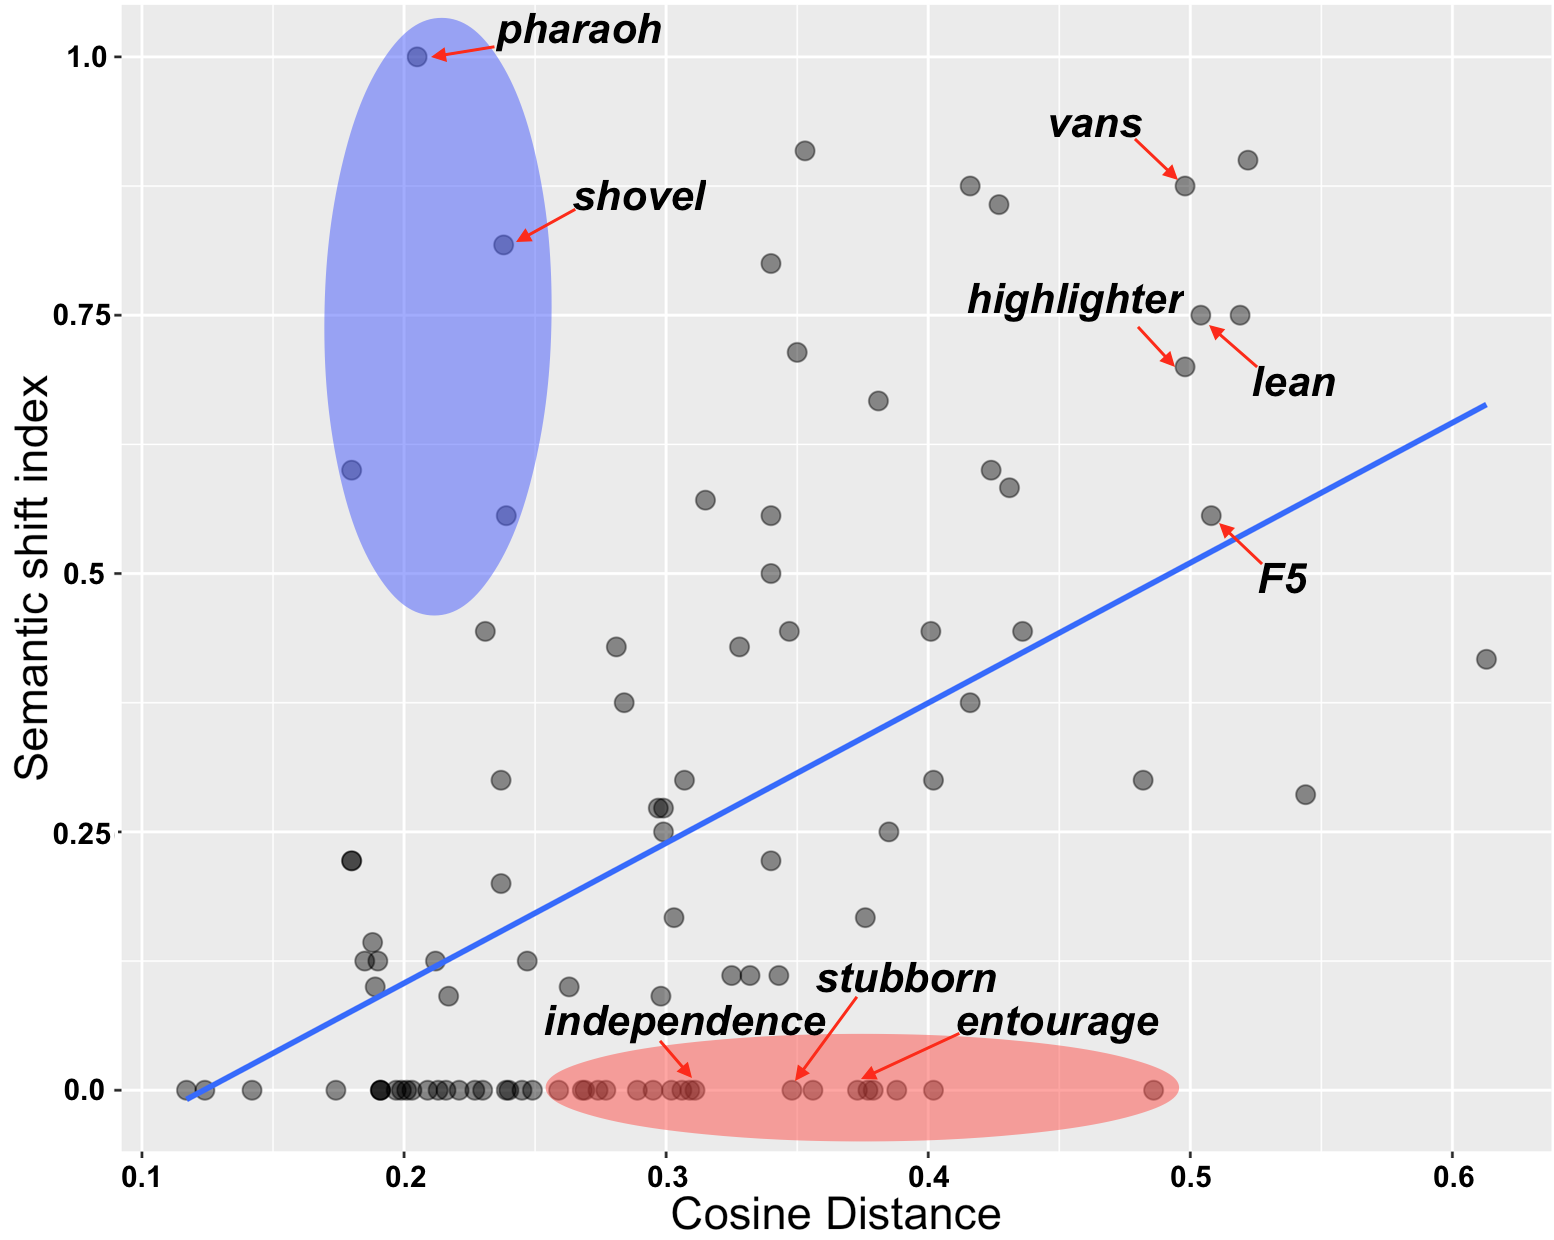
\includegraphics[width=\columnwidth]{images/cosine_distance_shift_index_annotated_3.png}
%\caption{Semantic shift index vs.~cosine distance for all words in the evaluation dataset (Pearson's $r$ = 0.49, $p< 0.001$). 
%Red ellipsis indicates false positives, blue ellipsis false
%negatives.
%\label{fig:shift-cosine}}
%\end{figure}

% RAQ's VERSION

\begin{figure}[t]\centering
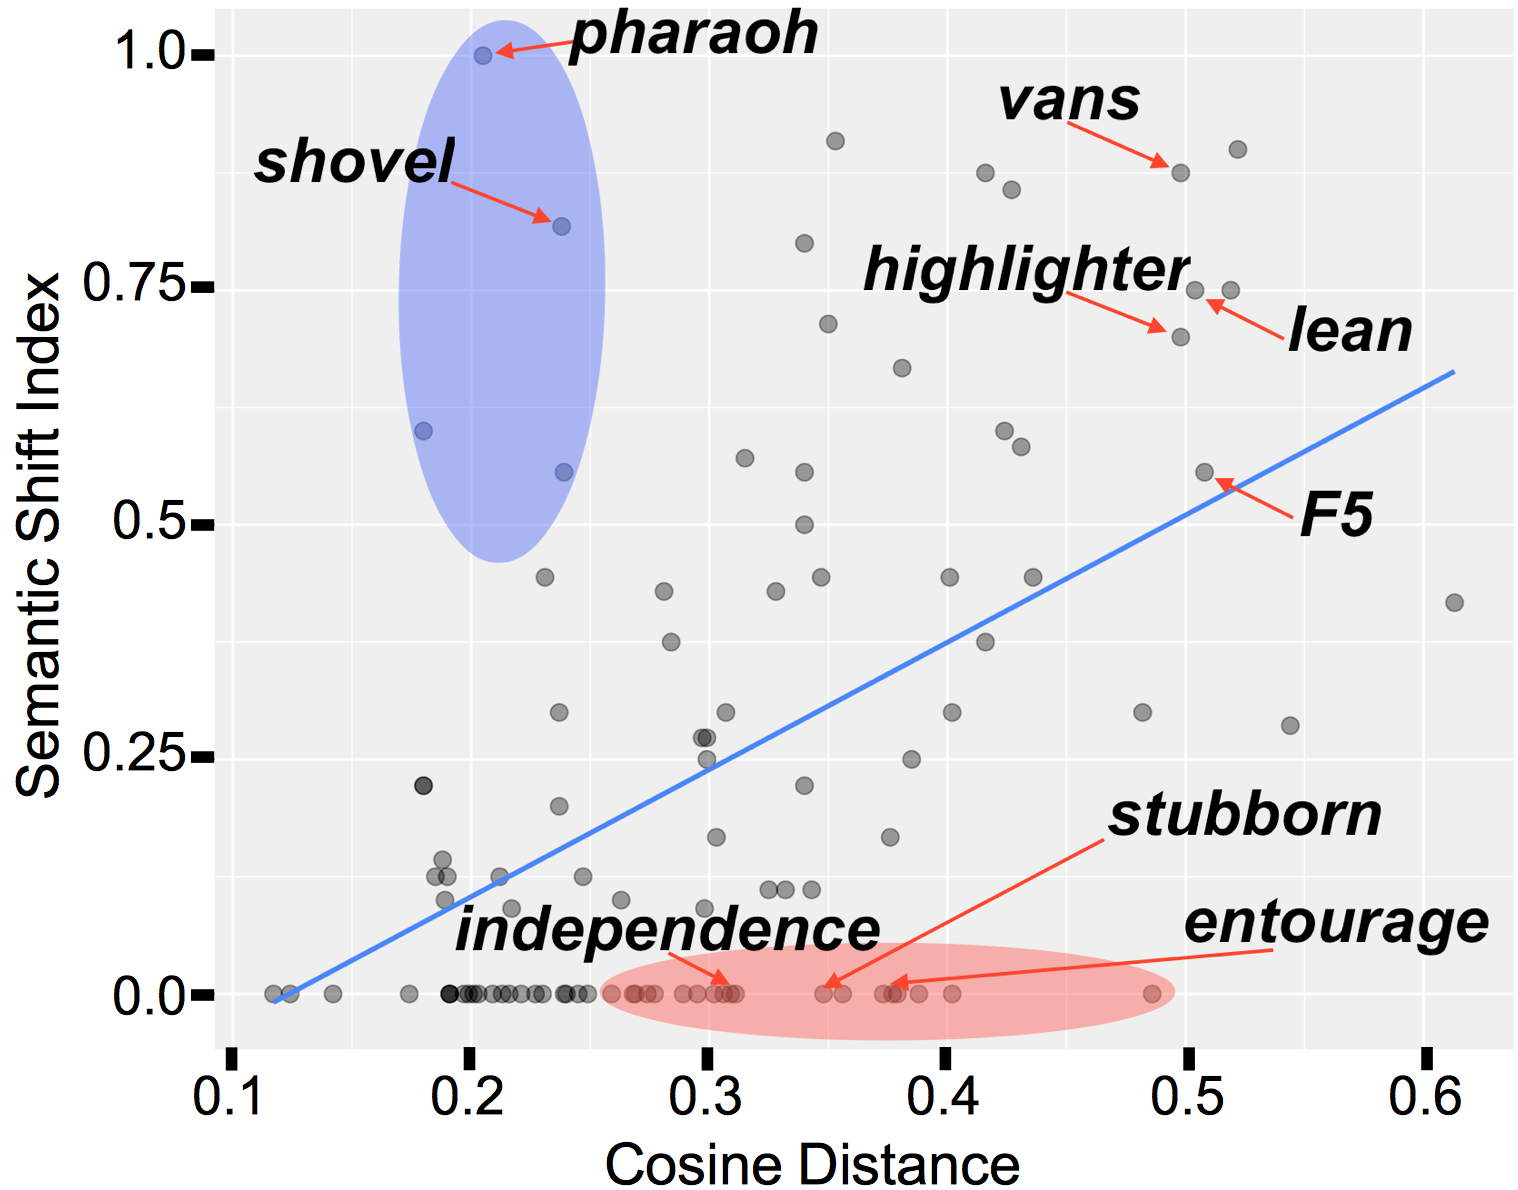
\includegraphics[width=\columnwidth]{images/cosine_distance_shift_index_annotated_6.png}
\caption{Semantic shift index vs.~cosine distance in the evaluation dataset (Pearson's $r$ = 0.49, $p< 0.001$). 
Red horizontal ellipsis:~false positives; blue vertical ellipsis:~false negatives.
\label{fig:shift-cosine}}
\end{figure}

%Our hypothesis that meaning shift is mirrored by an increased cosine distance between time-related word vectors is confirmed by the positive correlation between cosine distance and semantic shift (Pearson's $r$= 0.49, $p<0.001$) - see Figure \ref{fig:shift-cosine}. 
The positive correlation between cosine distance and semantic shift index (Pearson's $r$= 0.49, $p<0.001$, see Figure \ref{fig:shift-cosine}) confirms the hypothesis that meaning shift is mirrored by a change in context of use. However, we also find systematic deviations. 

%\paragraph{False negatives.}
\subsection{False negatives}
\label{subsec:False negatives}

A small, but consistent group is that of %\textit{false negatives}: 
words that undergo semantic shift but are not captured by the model
(blue vertical ellipsis Figure~\ref{fig:shift-cosine}; shift index\textgreater 0.5, cosine distance\textless 0.25).
These are all metaphorical shifts; in particular, cases of extended
metaphor \cite{werth1994extended}, where the metaphor is 
developed throughout the whole text.
%produced by an author. 
For instance, besides the {\em `shovel'} example mentioned in Section~\ref{sec:types}, we find {\em `pharaoh'}, the nickname of an Egyptian player who
joined Liverpool in 2017, used in
sentences like \textit{`approved by our new Pharaoh Tutankhamun'}, or \textit{`our dear Egyptian Pharaoh, let's hope he becomes a God'}.
Despite the metaphoric usage, the local context of these words is similar to the literal one, and so the model does not spot the meaning shift. We expect this to happen in long-term shift models, too, but we are not aware of results confirming this.

%\paragraph{False positives.}
\subsection{False positives}
\label{subsec:False positives}
A larger group of problematic cases is that of %\textit{false positives}, that is, 
words that do \textit{not} undergo semantic shift despite showing
relatively large differences in context between $t_1$ and $t_2$ (red horizontal ellipsis in
Figure~\ref{fig:shift-cosine}; shift index=0, cosine distance\textgreater	
0.25). Manual inspection reveals that most of these ``errors'' 
are due to a referential effect: words are used
almost exclusively to refer to a specific person or event in $t_2$, and
so the context of use is different from the contexts in $t_1$.
%\todo{M:this is dangerous, cause we do not prove this} 
For instance, {\em `stubborn'} is
almost always used to talk about a coach who was not
there in 2013 but only in 2017; 
{\em `entourage'}, for the entourage of a particular star of the team; {\em `independence'} for the
political events in Catalonia (Spain). 
In all these cases, the meaning of the word stays the same, %\todo{R: should we say the *ontological* meaning stays the same?} 
despite the change in context. In line with the Distributional
Hypothesis, the model spots the context change, but it is not
sensitive to its nature. We expect long-term shift to not be as
susceptible to referential effects 
like these because
embeddings are aggregated over a larger and more varied number of
occurrences.

We expect that in referential cases the contexts of use will 
%not simply be different, but 
be \textit{narrower} than for words with actual
semantic shift, as they are specific to one person or
event. Hence, a measure of \textit{contextual variability}
should help spot false positives.  To test this hypothesis, we define
contextual variability as follows: For a target word, we create a
vector for each of its contexts (5 words on both sides of the target) in $t_2$ by averaging the embeddings of
the words occurring in it, and define variability as the average
pairwise cosine distance between context vectors.%
\footnote{There are alternative ways of measuring contextual variability, but we expect them to yield the same picture.
For instance, we experimented with a different window size and obtained the same pattern.}
We find that
contextual variability is indeed significantly correlated with
semantic shift in our dataset (Pearson's $r\!=\!0.55$, $p\!<\!0.001$),
while it is independent from cosine distance (Pearson's $r$= 0.18,
$p> 0.05$). These two aspects are thus complementary. While both shift
words and referential cases change context of use in $t_2$, context
variability captures the fact that only in referential cases words
occur in a restricted set of contexts. 
%The scatterplot in
Figure~\ref{fig:shift-variability} shows this effect visually.  This
result can inform future 
%computational 
models of short-term meaning
shift.
% gbt: if anything, this should go in the conclusion, but I'd leave it out
% In future work, we plan to investigate more in depth the interplay between variability, cosine and semantic shift, both in short- and long-term meaning change.

\begin{figure}[h!]\centering
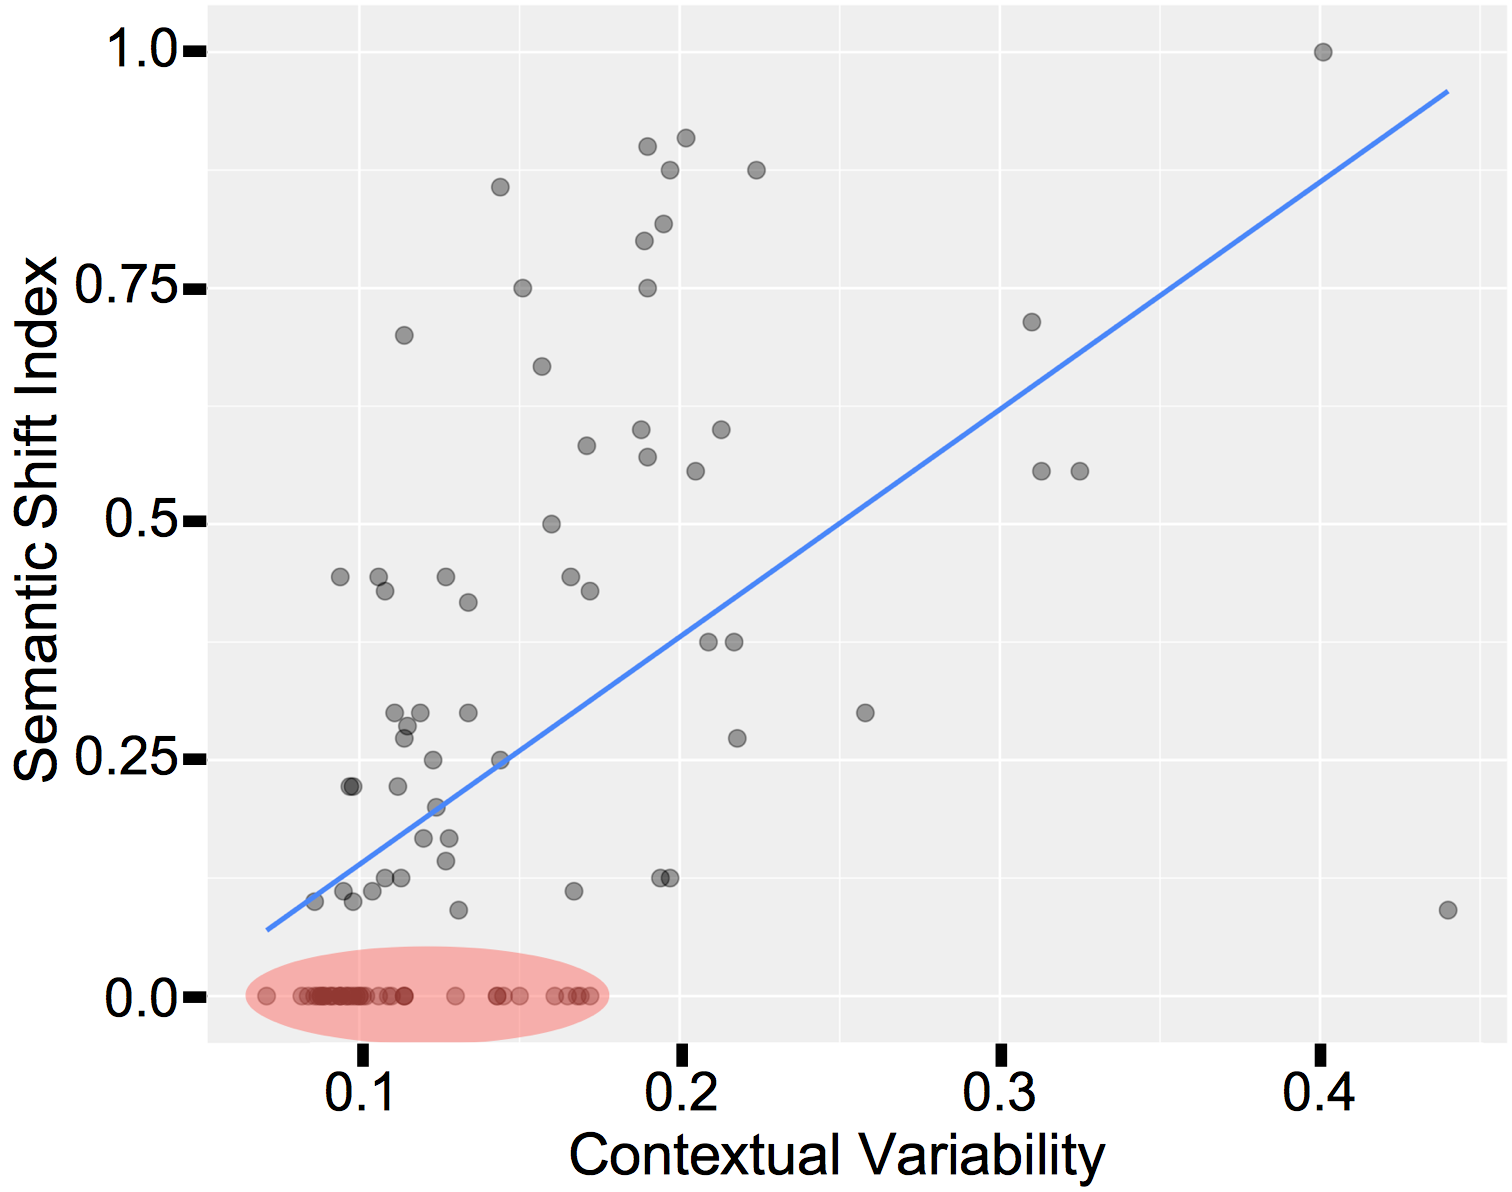
\includegraphics[width=\columnwidth]{images/contextual_variability_shift_index_annotated_4.png}
\caption{Semantic shift index vs.~context variability. Red horizontal ellipsis: referential cases which are assigned high cosine distance values by the model (false positives).\label{fig:shift-variability}}
\end{figure}


%\begin{figure}[t]\centering
%%\includegraphics[width=\columnwidth]{graph_and_csv/plots/shift-cosine-correlation-plot.png}
%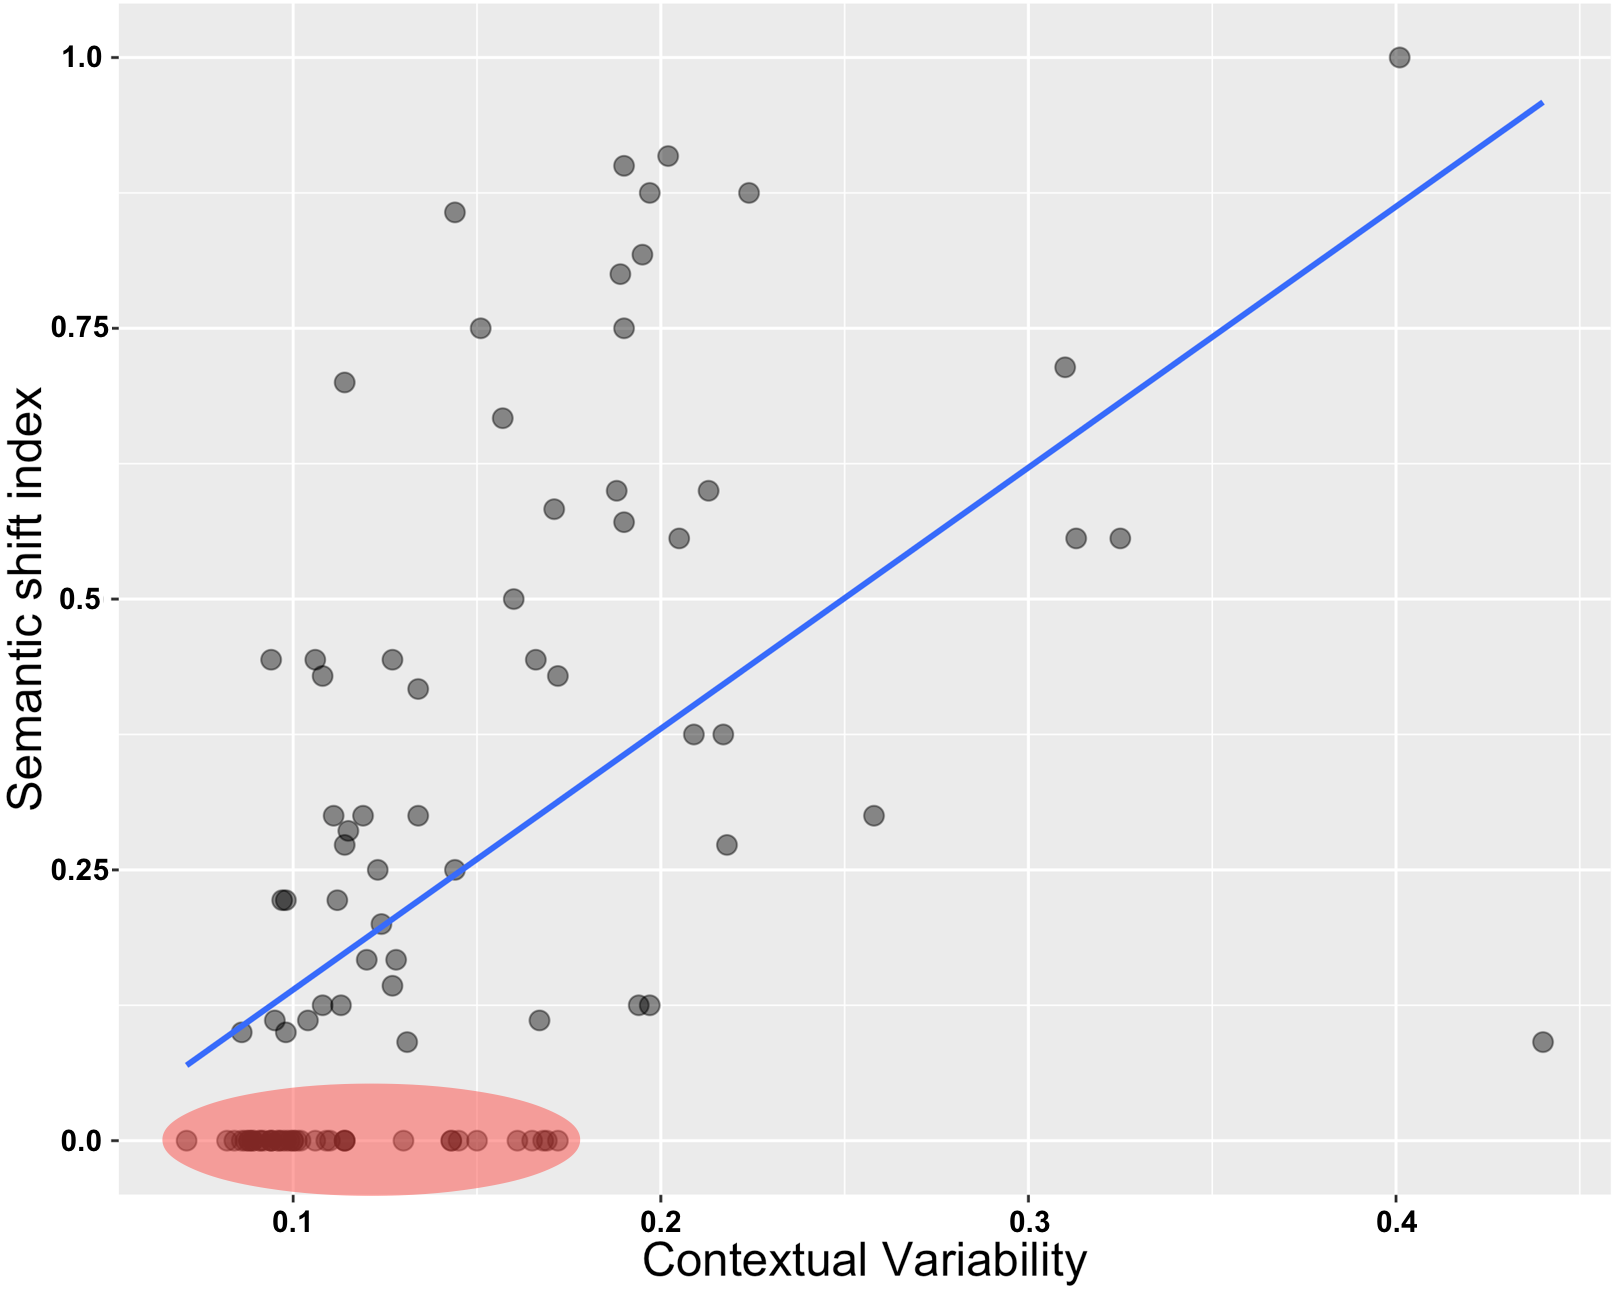
\includegraphics[width=\columnwidth]{images/contextual_variability_shift_index_annotated_2.png}
%\caption{Semantic shift index vs.~context variability for all words in the evaluation dataset (Pearson's $r$ = 0.55, $p< 0.001$). Red ellipses indicates the referential cases which are assigned high cosine distance values by the model (false positives).
%\label{fig:shift-variability}}
%\end{figure}


%




%% PREVIOUS VERSION


%Although the general tendency is in line with our expectations, we
%also find systematic deviations. First, \textit{false positives}, that
%is, words that do not undergo semantic shift despite showing
%relatively large differences in context between $t_1$ and $t_2$ (red ellipsis in
%Figure~\ref{fig:shift-cosine}; shift index=0, cosine distance\textgreater	
%0.25). 
%%\todo{G Redraw red ellipsis to cover fewer datapoints -- maybe  higher than 0.25? Else too close to the 0 x-axis.}
%Manual inspection reveals that most of these ``errors'' 
%%\todo{Add  number (X out of Y)?} 
%are due to a referential effect: words are used
%% \paragraph{False Positives.}
%% The analysis of words in this group reveals that, indeed, they occur
%% in a different context in $t$ 2 compared to  $t$ 1: however, this not
%% due to a meaning shift, but rather to the fact that they are used 
%almost exclusively to refer to a specific person or event, and
%so the context of use is narrowed down with respect to $t_1$.
%%\todo{M:this is dangerous, cause we do not prove this} 
%For instance, `stubborn' is
%almost always used to talk about a coach who was not
%there in 2013 but only in 2017; 
%%`village', for the village in Africa where one of the new players comes from; 
%`entourage', for the entourage of one of the stars of the team; `independence' for the
%political events of Catalonia (Spain). 
%%\todo{do we want to include the example  of `parked'?}. 
%% the target word is temporary
%% narrowing down its context of use to refer to a specific referent, but
%% without a semantic shift.
%In all these cases, the meaning of the word stays the same, despite
%the change in context. In line with the Distributional Hypothesis, the model spots the change, but it is not sensitive to its nature.
%Long-term shift is not as sensitive to changes of referential nature
%like these because
%embeddings are aggregated over a larger and more varied number of
%occurrences.
%%However, with small time-scales and in-community semantic shift, this problem clearly emerges.
%
%%\raq{To structure this, now I would add two subheadings (with paragraph command) for false positive and false negatives and put the explanations/examples you have below for each of them.}
%
%
%A smaller, but consistent group is that of \textit{false negatives}, 
%words that undergo semantic shift but are not captured by the model
%(blue ellipsis; shift index\textgreater 0.5, cosine distance\textless 0.25).
%%: `dilly', `shovel', `shovels', `pharaoh'.\todo{M: dont't think list is necessary}
%%\gbt{List the  words here, since they are only 4.}
%%\paragraph{False Negatives.}
%%On the top left of the plot cluster cases that can be considered as
%%\textit{false negatives}, i.e. words that are considered cases of
%%semantic shift by the redditors (high semantic shift index values),
%%but not by the model (low cosine distance). 
%\gbt{To do: move this to the ling analysis section, and here only link?} \marco{don't know, I see it more here maybe. Raq?}
%These are cases of \textit{extended}
%metaphor \cite{werth1994extended}, that is, cases in which the metaphor is 
%%not limited to a single word, but it is 
%developed throughout the whole text produced by an author. Also in this case, the model ``is right'', in the sense that indeed
%the local context of the target words does not change in $t_2$.
% % As a result, the context taken into consideration by the model is
% % indeed the one in which the word normally occurs, and for this
% % reason the model is not able to spot the meaning shift. 
%For instance, `pharaoh' is the nickname of an Egyptian player who
%joined Liverpool in 2017 and is used in
%sentences like \textit{`approved by our new \textbf{Pharaoh}
%  Tutankhamun'}, \textit{'our dear Egyptian \textbf{Pharaoh},
%  let's hope he becomes a God'}, and so on. Similarly, `shovel',  occurs in sentences
%like \textit{`welcome aboard, here is your \textbf{shovel}'},
%\textit{`you boys know how to \textbf{shovel} coal'}: the team is seen as a train that is running through the season, and every supporter is asked to give its contribution, depicted as the act of shoving coal into the train boiler. Despite the metaphoric usage, the local context of these words is similar to the literal one, and so the model does not spot the meaning shift. We expect this to happen in long-term shift models, too, but we are not aware of results confirming this.
%



%\section{Contextual variability}
%
%From the analysis it emerges that the main issue for distributional models when dealing
%with short-term shift is contextual change due to referential aspects (false positives).
%We expect that in referential cases the context of use will be
%\textit{narrower} than for words with actual semantic shift, because
%they are specific to one person or event. Hence, using a measure of
%\textit{contextual variability} should help spot false
%positives.
%Here we test this hypothesis. 
%We define contextual variability as follows: for a target word, we create a vector for each of its contexts in $t_2$ by averaging the embeddings of the words  occurring in it, and define variability as the average pairwise cosine distance between context vectors.\footnote{We consider the context as the five words occurring on the left and on the right of the target word.}We then test whether contextual variability has explanatory power over cosine distance by fitting a linear regression model with these two variables as predictors and semantic shift index as dependent variable.\footnote{Contextual variability and cosine distance are not correlated in our data (Pearson's $r$= 0.18,$p> 0.05$). }
%The results indicate that these two aspects are indeed complementary
%(contextual variability: $\beta$= 0.47, $p< 0.001$, cosine distance:
%$\beta$= 0.40, $p< 0.001$, adjusted $R^2$=0.44). While both shift
%words and referential cases change context of use in $t_2$, context
%variability captures the fact that only in referential cases words
%occur in a restricted set of contexts. The scatterplot
%\ref{fig:shift-variability} shows this effect visually. \new{This result can inform future models of short-term meaning
%  shift.} \textcolor{red}{In future work, we plan to investigate more in depth the interplay between variability, cosine and semantic shift, both in short- and long-term meaning shift.}\marco{I'd move this to Conclusions}



%%% Local Variables:
%%% mode: latex
%%% TeX-master: "main"
%%% End:
